%% 
%% Copyright 2019-2021 Elsevier Ltd
%% 
%% This file is part of the 'CAS Bundle'.
%% --------------------------------------
%% 
%% It may be distributed under the conditions of the LaTeX Project Public
%% License, either version 1.2 of this license or (at your option) any
%% later version.  The latest version of this license is in
%%    http://www.latex-project.org/lppl.txt
%% and version 1.2 or later is part of all distributions of LaTeX
%% version 1999/12/01 or later.
%% 
%% The list of all files belonging to the 'CAS Bundle' is
%% given in the file `manifest.txt'.
%% 
%% Template article for cas-sc documentclass for 
%% single column output.

% Document Class
\documentclass[a4paper,fleqn]{cas-sc}

% Packages
\usepackage[authoryear,longnamesfirst]{natbib}

%Package to Figure
\usepackage{float}	% permite posicionar a figura entre parágrafos usando H

%Author macros
\def\tsc#1{\csdef{#1}{\textsc{\lowercase{#1}}\xspace}}
\tsc{WGM}
\tsc{QE}

\begin{document}
\let\WriteBookmarks\relax
\def\floatpagepagefraction{1}
\def\textpagefraction{.001}

% Short title
\shorttitle{Transverse gallery of twin tunnels}    

% Short author
\shortauthors{Quevedo et al.}  

% Main title of the paper
\title [mode = title]{Numerical analysis of the twin tunnels with transverse galleries using plastic and viscous 
	constitutive models for rockmass and lining}  

% First author
\author[1]{Quevedo, F. P. M.}[style = chinese, orcid = 0000-0003-4171-1696]
\cormark[1] 					
\cortext[cor1]{Corresponding author.}
\ead{motta.quevedo@ufrgs.br}
\ead[url]{https://www.researchgate.net/profile/Felipe-Pinto-Da-Motta-Quevedo}

% Second author
\author[1]{Colombo, C. A. M. M.}[style=chinese, orcid=0000-0000-0000-0000]
\ead{carlos.colombo@ufrgs.br}
\ead[url]{http://lattes.cnpq.br/4919388217690564}

% Third author
\author[1]{Bernaud, D.}[style=chinese, orcid=0000-0001-6365-3269]
\ead{denise.bernaud@ufrgs.br}
\ead[url]{http://lattes.cnpq.br/2809615143819128}

% Four author
\author[1]{Maghous, S.}[style=chinese, orcid=0000-0002-1123-3411]
\ead{samir.maghous@ufrgs.br}
\ead[url]{http://lattes.cnpq.br/6305244914209829}

% Afilliation
\affiliation[1]{organization={Federal University of Rio Grande do Sul},
	addressline={Av. Osvaldo Aranha, 99}, 
	city={Porto Alegre},
	postcode={90.035-190}, 
	state={RS},
	country={Brazil}}

% Mathematical Symbols
%\newcommand{\All}{\boldsymbol A}
%\newcommand{\al}{\boldsymbol a}
%\newcommand{\bl}{\boldsymbol b}
%\newcommand{\Bll}{\boldsymbol B}
%\newcommand{\dfds}{\boldsymbol{f_\sigma}}
%\newcommand{\dfdq}{{f_q}}
\newcommand{\dgds}{\boldsymbol{g_\sigma}}
%\newcommand{\dPhidsl}{\boldsymbol{\Phi_{_\sigma}}}
%\newcommand{\dPhidql}{\boldsymbol{\Phi_{_q}}}
\newcommand{\Dll}{\boldsymbol{D}}
\newcommand{\Dllmod}{\boldsymbol{D^{*}}}
\newcommand{\Dllepvp}{\boldsymbol{D}^{epvp}}
%\newcommand{\Dsdep}{\boldsymbol{D}^{ep}}
%\newcommand{\Dsdev}{\boldsymbol{D}^{vp}}
%\newcommand{\Dsdepev}{\boldsymbol{D}^{epvp}}
\newcommand{\dstrain}{\boldsymbol{\dot{\varepsilon}}}
\newcommand{\dstraine}{\boldsymbol{\dot{\varepsilon}}^{e}}
\newcommand{\dstrainp}{\boldsymbol{\dot{\varepsilon}}^{p}}
\newcommand{\dstrainv}{\boldsymbol{\dot{\varepsilon}}^{vp}}
%
\newcommand{\straineqp}{\bar \varepsilon^p}
\newcommand{\dstrainsh}{\boldsymbol{\dot{\varepsilon}}^{sh}}
\newcommand{\dstraincr}{\boldsymbol{\dot{\varepsilon}}^{cr}}
%
\newcommand{\dstress}{\boldsymbol{\dot{\sigma}}}
%\newcommand{\Fl}{\boldsymbol{F}}
%\newcommand{\fvp}{f^{vp}}
%\newcommand{\gvp}{g^{vp}}
%\newcommand{\gllum}{\boldsymbol {g_{_1}}}
%\newcommand{\glldois}{\boldsymbol {g_{_2}}}
%\newcommand{\glltres}{\boldsymbol {g_{_3}}}
%\newcommand{\hl}{{h_q}}
%\newcommand{\Kll}{\boldsymbol K}
%\newcommand{\Nll}{\boldsymbol N}
\newcommand{\onell}{\boldsymbol{1}}
%\newcommand{\onellll}{\boldsymbol{I}}
%\newcommand{\Rl}{\boldsymbol{R}}
%\newcommand{\sll}{\boldsymbol{s}}
\newcommand{\strain}{\boldsymbol{\varepsilon}}
\newcommand{\straine}{\boldsymbol{\varepsilon}^{e}}
\newcommand{\strainp}{\boldsymbol{\varepsilon}^{p}}
\newcommand{\strainvp}{\boldsymbol{\varepsilon}^{vp}}
%\newcommand{\strainpeq}{\bar \varepsilon^p}
%\newcommand{\strainvpeq}{\bar \varepsilon^{vp}}
\newcommand{\stress}{\boldsymbol{\sigma}}
%\newcommand{\ul}{\boldsymbol u}
\newcommand{\zerol}{\boldsymbol 0}
%%
%%
%% Mathematical Symbols
%\newcommand{\deviator}{\boldsymbol{s}}
%\newcommand{\Disoliel}{\boldsymbol{D}}
%\newcommand{\Disolielmod}{\boldsymbol{D^{*}}}
%
%\newcommand{\dstraineq}{\dot{\bar{\varepsilon}}}
%
%\newcommand{\dstrainvp}{\boldsymbol{\dot{\varepsilon}}^{vp}}
%
%\newcommand{\flowtensorf}{\frac{\partial\fvp}{\partial\stress}}
%\newcommand{\flowtensorg}{\frac{\partial\gvp}{\partial\stress}}
%\newcommand{\fo}{f_0}
%
%\newcommand{\Jtwo}{J_{2}}
%\newcommand{\onefour}{\boldsymbol{I}}
%\newcommand{\qvp}{\boldsymbol{q}^{vp}}
%\newcommand{\sphericaltensor}{\boldsymbol{1}\otimes\boldsymbol{1}}
%
\newcommand{\straincr}{\boldsymbol{\varepsilon}^{cr}}
%
\newcommand{\strainsh}{\boldsymbol{\varepsilon}^{sh}}
\newcommand{\strainshCEB}{\varepsilon_{sh}}
%
%\newcommand{\stresseq}{\bar{\sigma}}
%\newcommand{\stressy}{\sigma_{y}}
%\newcommand{\unitarytensor}{\boldsymbol{1}}
%\newcommand{\young}{E}

% Here goes the abstract
\begin{abstract}
This paper aims to demonstrate the long-term implications of the rheological constitutive behavior of rock mass and concrete lining in the convergence of the intersection area of twin tunnel galleries using a three-dimensional numerical analysis based on the finite-element method. A Drucker-Prager-Perzyna elastoplastic-viscoplastic constitutive law represents the rock mass and, for the lining, an elastic and viscoelastic law. The deactivation-activation methods simulate the excavation process. Comparisons of convergence reveal that the viscous effects of the rock mass and the lining significantly influence the peak convergence within the intersection zone, resulting in differences of approximately 10\% in convergence values.
%É necessário um resumo conciso e factual. O resumo deve indicar sucintamente o objetivo da investigação, os principais resultados e as principais conclusões. O resumo é frequentemente apresentado separadamente do artigo, pelo que deve ser autónomo. Por esta razão, as referências devem ser evitadas, mas se forem essenciais, devem citar-se o(s) autor(es) e o(s) ano(s). Além disso, devem ser evitadas abreviaturas não padronizadas ou pouco comuns, mas se forem essenciais, devem ser definidas na primeira menção no próprio resumo. Os artigos com "Sugestões de Métodos" não devem conter resumos.
\end{abstract}

% Use if graphical abstract is present
%\begin{graphicalabstract}
%\includegraphics{}
%\end{graphicalabstract}

% Research highlights
\begin{highlights}
	\item Qualquer coisa 1
	\item Qualquer coisa 2
	\item Qualquer coisa 3 
\end{highlights}

% Keywords
\begin{keywords}
twin tunnels \sep transverse gallery \sep constitutive models \sep finite element method
\end{keywords}

\maketitle

\section{Introduction}\label{}

The structural design of deep twin tunnels involves estimating cross-section convergence, lining pressure, and the size of the plastic zone within the rock mass caused by the excavation process. The final convergence and stress field around the tunnel depend on \textit{in situ} initial stresses, cross-section geometry, and the coupling between the lining and the rock mass during construction. Unlinke a single tunnel, the proximity between twin tunnels break the symmetry of deformations in tunnel wall. Many twin tunnels have transverse galleries that serve as emergency routes. These galleries will introduce a local effect on the convergence profile of the longitudinal tunnel. 

Additionaly, the rheological behavior of the rockmass and lining plays a crucial role in how stress and displacements fields evolve over time.

%Many studies have proposed viscous constitutive models for the rock mass. Some of these models use instantaneous linear elastic behavior. However, more and more studies have analyzed the impact of instantaneous elastoplastic behavior with viscous long-term components [\citenum{rousset1988}, \citenum{piepi1995}, \citenum{Purwodihardjo2003}, \citenum{Kleine2007}, \citenum{Shafiqu2008}, \citenum{Barla2010}, \citenum{souley2011}, \citenum{Manh2015}]. Incorporating elastoplastic behavior has a more apropriate representation of rock mass since the stress state can reach plasticity during excavation. These coupled models are better in regions with high-stress deviations where plasticity-induced stress redistribution will impact the viscous component.

%Despite these developments, there are few studies about the interaction of the rheological behavior of the lining with viscous rock mass [\citenum{pottler1990}, \citenum{meschke1996}, \citenum{mavsin2009}, \citenum{NEUNER2021}]. Thus, the aim of this study is to investigate the influence of some of the main parameters of deep concrete-lined tunnels in long-term convergence.


Indicar os objectivos do trabalho e fornecer um contexto adequado, evitando uma pesquisa bibliográfica
ou um resumo dos resultados.


\section{Statement of problem and fundamental assumptions}\label{}

%The results of this study apply only when the following hypotheses are satisfied:

%\begin{enumerate}[(a)]

%\item tunnel with circular cross section;
%\item full, flat, and vertical excavation face without using presupport
%techniques;
%\item constant excavation speed;
%\item homogeneous concrete lining with constant section;
%\item initial state of hydrostatic radial stresses and constant normal
%stress equal to the radial stresses along the depth;
%\item the rock mass must have a perfect viscoplastic behavior, independent of hydrostatic stresses;
%\item constant humidity and temperature in the concrete lining during
%the creep evolution;
%\item perfect adhesion (rigid contact) between lining and rock mass
%interface;
%\item concrete lining stress level below 40\% of the average compressive strength; this is limited so that the superposition principle of
%the CEB-FIP MC90 creep model remains valid.
%	
%\end{enumerate}	

\section{Constitutive Model of the Rock Material}\label{}

An elastoplastic-viscoplastic constitutive model was implemented in ANSYS using the UPF/USERMAT customization tool [\citenum{ANSYS:2013b}] to simulate rock mass.  This model concern a serial association of the plastic and viscoplastic constitutive models, i.e., the total strain $\dstrain = \dstraine + \dstrainp + \dstrainv$, which leads to the following linear constitutive relationship:
\begin{equation} \label{eq_constitutive_relationship_epvp}
	\dstress = \Dll : \dstraine = \Dll : (\dstrain - \dstrainp - \dstrainv),\;
\end{equation}
where $\dstraine$, $\dstrainp$ and $\dstrainv$, represent the elastic, plastic and viscoplastic strain rate, respectively. The one-dimensional representation in Fig.~\ref{reological_scheme} shows this association. 

\begin{figure}
	\centering
	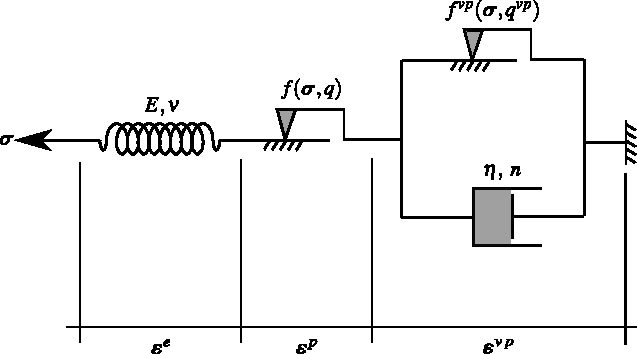
\includegraphics[scale=1]{Rheological representation.pdf}
	\caption{Rheological representation of the elastoplastic-viscoplastic model.}
	\label{reological_scheme}
\end{figure}
In this model is used a Drucker-Prager plastic flow surface given by
\begin{equation}
	\label{eq:f_Drucker_Prager}
	f(\stress,q) = f(I_1,J_2,q) = \beta_1 I_1 +\beta_2 \sqrt{J_2}-q(\alpha),
\end{equation}
which $I_1$ is the first invariant of the stress tensor, $J_2$ the second invariant of the deviator tensor and $\beta_1, \beta_2$ and $q(\alpha)$ are strength parameters related to the friction angle $\phi$ and cohesion $c(\alpha)$, respectively. In the present model Drucker-Prager surface been inner of the Mohr-Coulomb surface [\citenum{bernaud1991}], that is,
\begin{equation}
	\label{eq:f_DP_inscrita_MC}
	\beta_1 = \dfrac{(k-1)}{3}, ~~~ \beta_2 = \dfrac{(2k+1)}{\sqrt{3}}, ~~~
	q(\alpha) = 2\sqrt{k}~c(\alpha),
\end{equation}
where $k = (1+\sin{\phi})/(1-\sin{\phi})$. The internal variable $\alpha$ is the equivalent plastic strain $\straineqp$ used to simulate strain hardening/softening phenomena. However, for this study, we adopt perfect plasticity, meaning that c is a constant. For the viscoplasticity surface $f^{vp}$ the same surface is empolyed, but with $\phi^{vp}$ in $\beta_1$ and $\beta_2$, and $q^{vp} = 2\sqrt{k^{vp}}-c^{vp}$ where $k^{vp} = (1+\sin{\phi^{vp}})/(1-\sin{\phi^{vp}})$ and $c^{vp}$ is a constant, i.e., perfect viscoplasticity. 

The plastic flow rule is given by:
\begin{equation}
	\label{eq_plastic_flow}
	\dot \strainp = \left\{ 
	\begin{array}{ll} 
		\dot \lambda \dfrac{\partial g}{\partial \stress} &  \text{for } f > 0 \\ 
		\zerol, & \text{for } f < 0 \\
	\end{array}\right.,
\end{equation}
where $\dot \lambda$ is the plasticity multiplier and $g$ is a potencial flow analogous to $f$ to simulate the volume dilatation during the evolution of plastic deformations. However, for this analysis, was used associated plasticity, i.e., $g=f$. The plastic multiplier is obtained through the consistency condition $\dot f = 0$. Numerical details of this implementation can be found in [\citenum{quevedo2022b}]. For viscoplastic flow rule we have,
\begin{equation}
	\label{eq_viscoplastic_flow}
	\dstrainv = \dot \lambda^{vp} \dfrac{\partial f^{vp}}{\partial \stress}
\end{equation}
In contrast to the plastic multiplier, the viscoplastic multiplier is independent of a consistency condition. As a result, its expression is explicit. For this study, we utilize the Perzyna model as follows:
\begin{equation} \label{eq_perzyna_model}
	\dot \lambda^{vp} = \dfrac{\Phi(\stress,q^{vp})}{\eta}~~~\text{and}~~~\Phi = \left\langle  \dfrac{f^{vp}(\stress,q^{vp})}{f_0} \right\rangle^n, \,
\end{equation} where $\Phi$ is the overstress function, $\eta$ is the dynamic viscosity constant, $n$ is the dimensionless parameter that gives the form of the power law, $f_0$ a parameter conveniently adopted and $\left\langle * \right\rangle$ is the McCauley function which is $0$ when $* <0$ , i.e. viscoplastic flow will only occur when the overstress function is positive.

In this coupled model, when $\phi=\phi^{vp}$, cohesion entirely controls the evolution of local mechanical fields. Specifically, when  $c \rightarrow \infty$ and $c^{vp} \rightarrow \infty$, the system achieves a purely elastic solution. The solution becomes purely elastoviscoplastic with $c \rightarrow \infty$, while a pure elastoplastic solution emerges with $c^{vp} \rightarrow \infty$. In this study's coupled analysis, we have adopted $c^{vp} < c$, allowing the viscoplastic domain to occur independently of plasticity. However, in the presence of plasticity, viscous effects become inevitable. Fig.~\ref{epvpdomains} illustrates these domains in principal stress space.
\begin{figure}
	\centering
	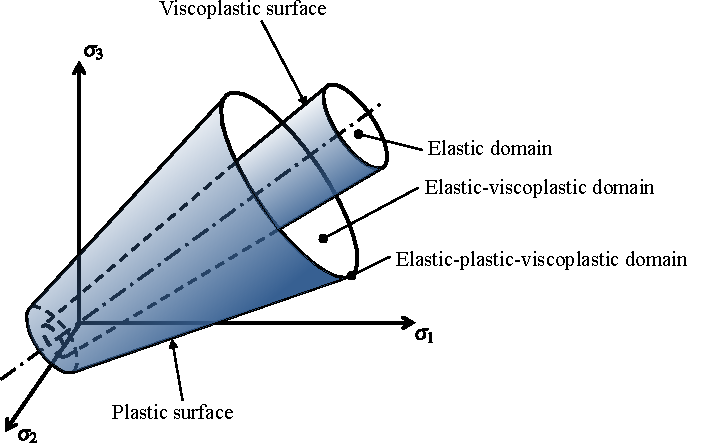
\includegraphics[scale=0.8]{Elastic-plastic-viscoplastic domains.pdf}
	\caption{Elastoplastic-viscoplastic domains.}
	\label{epvpdomains}
\end{figure}

Details of this model, including validations and its application in single tunnel, are in [\citenum{quevedo2022b}]. See [\citenum{quevedo2022thesis}] for the algorithm details implemented in FORTRAN within the USERMAT subroutine.

\section{Constitutive Model of the Lining}\label{}

We implemented a viscoelastic model in ANSYS using the UPF/USERMAT customization feature [\citenum{ANSYS:2013b}]. The model simulates concrete creep through a Generalized Kelvin chain, based on Bažant and Prasannan's Solidification Theory [\citenum{bazant:1989a,bazant:1989b}], with parameter adjustments performed using the CEB-FIP MC90 formulation. The CEB-FIP MC90 formulation also [\citenum{CEB:1993}] determines the shrinkage component. 

In this model, the constitutive relationship between stress and strain is 
\begin{equation} \label{eq:8}
	\dstress = \Dll : \dstraine = \Dll : \dstrain - \Dll : \dstrainsh - \Dllmod : \dstraincr\;
\end{equation}
where $\dstrainsh$  and $\dstraincr$ are the shrinkage and creep strain rate, respectively, while $\Dllmod$ denotes the modified constitutive tensor that incorporates the aging of the concrete. Due to the time integration scheme for Newton-Raphson algorithm, the Eq.~(\ref{eq:8}) is given by:
\begin{equation} \label{eq:9}
	\stress_{n+1} = \stress_{n}+\Dll : \Delta \strain - \Dll : \Delta \strainsh - \Dllmod : \Delta \straincr \;
\end{equation}
in which the increment of shrinkage strain is:
\begin{equation} \label{eq:10}
	\Delta \strainsh =  \Delta \strainshCEB(t_{s}) \onell \;
\end{equation}
where $t_{s}$ represents the concrete curing time, and $\Delta \strainshCEB$ is the variation of magnitude of the concrete deformation by shrinkage, determined using the expressions of CEB-FIP MC90 [\citenum{CEB:1993}]. To calculate the increment of creep strain, denoted as $\Delta \straincr$, we use the incremental algorithm developed by Bažant and Prasannan [\citenum{bazant:1989a,bazant:1989b}], with an adjustment to incorporate CEB-FIP MC90 formulation. This adaptation is possible comparing the creep functions $J(t,t_0)$ of both references. This gives to the following equivalence:
\begin{equation} \label{eq:11}
	E_0 = E_c(t_0),~ \gamma_c(t-t_0)=\beta_c(t-t_0),~ \frac{1}{v(t)} = \frac{\phi_0}{E_{ci}} \text{  and  } \frac{1}{\eta(t)}=0 \;
\end{equation}
in which, according to Bažant and Prasannan [\citenum{bazant:1989a,bazant:1989b}], $E_0$  is the modulus of elasticity of the concrete aggregates and microscopic particles of the cement paste, $\gamma_c(t-t_0)$ is the microviscoelastic deformation of the volume fraction of solidified concrete $v(t)$, $\eta(t)$ is the apparent macroscopic viscosity and, according to CEB-FIP MC90 [\citenum{CEB:1993}], $E_c(t_0)$ is the tangent elastic modulus of the concrete at the instant of loading application $t_0$, $\beta_c(t-t_0)$  is a coefficient that depends on the loading age $t-t_0$ , $\phi_0$ is a coefficient that depends on the age of the concrete at the instant of loading application and $E_{ci}$  the tangent elasticity modulus of the concrete at the age of 28 day.


Details of this model, including validations and its application in single tunnel, are in [\citenum{quevedo2022}]. See [\citenum{quevedo2017comportamento}] for the algorithm details implemented in FORTRAN within the USERMAT subroutine.


\section{Numerical model}\label{}

The spatial discretization of the domain corresponds to a mesh with trilinear hexahedral elements (SOLID 185), except in the gallery region, which uses higher-order tetrahedral elements (SOLID186). Fig.~\ref{Mesh1} shows the mesh, geometric parameters, and boundary conditions for the problem in question. In this figure, $d1$ is the distance between longitudinal tunnel axes, $R_i$ longitudinal tunnel cross-section radius, $L_2$ total excavated length, $d_3$ domain height, $L_1$ length of the unexcavated region, $L_3$, $L_p$ step length of the excavation process, $d_2$ position of the gallery along the longitudinal tunnel.

\begin{figure}
	\centering
	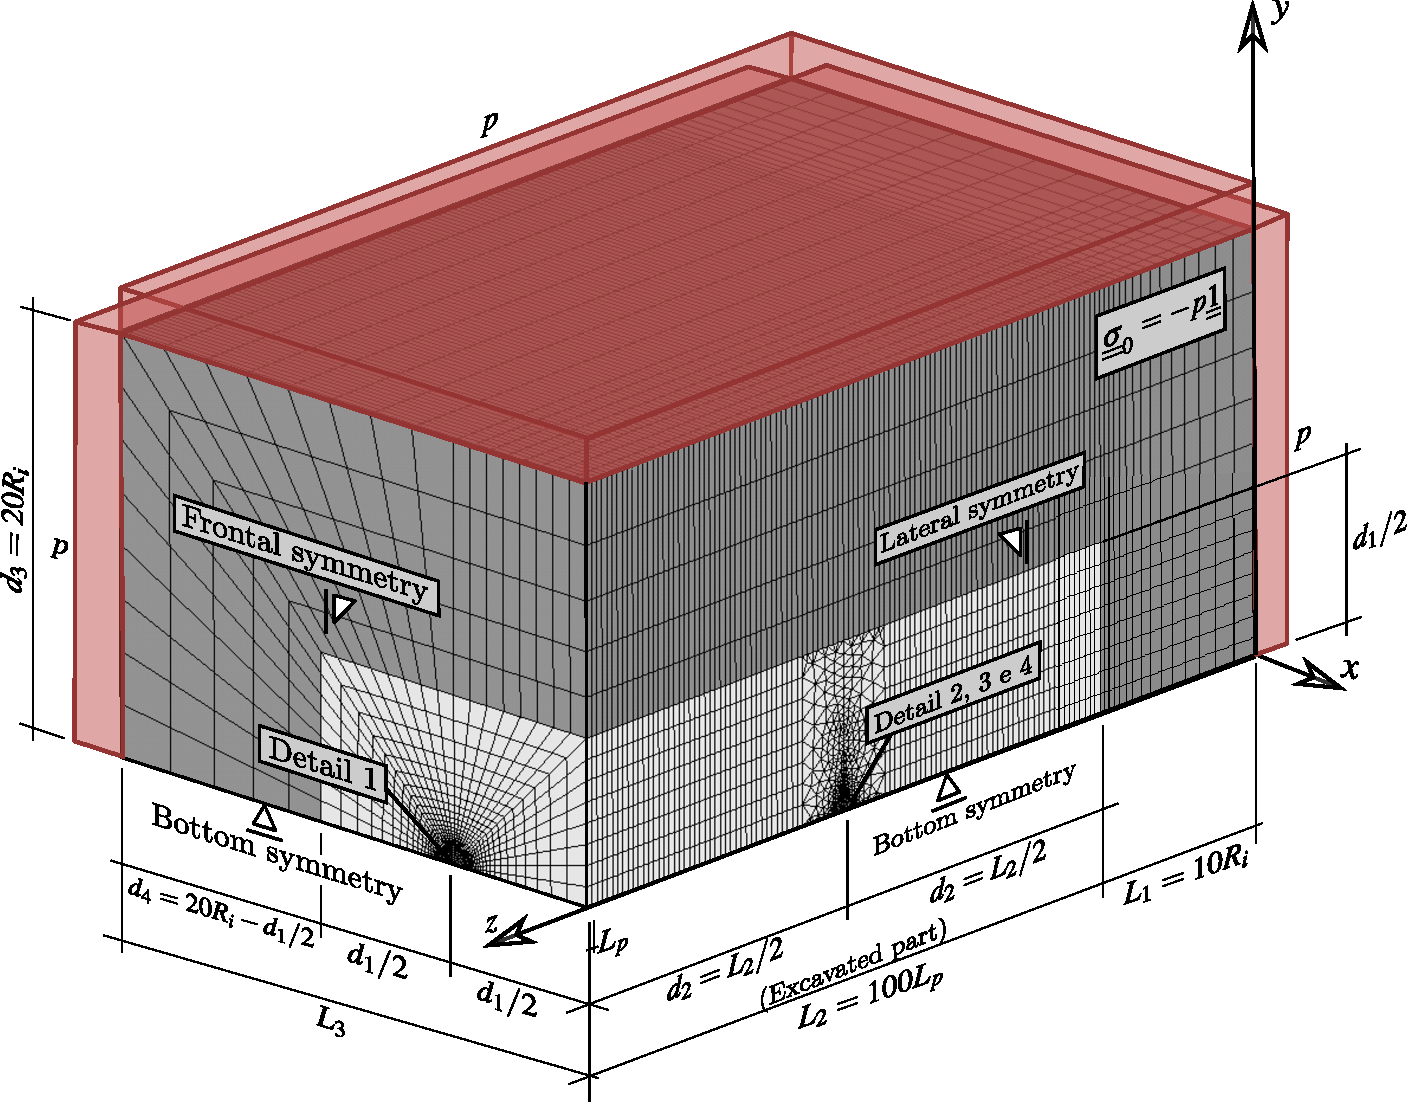
\includegraphics[scale=0.5]{Mesh1.pdf}
	\caption{Mesh, dimensions and boundary conditions of the 3D twin tunnel domain}
	\label{Mesh1}
\end{figure}


We considered front, side, and bottom symmetry to reduce computational cost. In conjunction with boundary pressure $p$, we apply the initial stress condition $\sigma_0$ at all integration points to simulate the initial state of an undisturbed rock mass, i.e., a zero deformation field before excavation begins. We checked the vertical distortion of the elements away from the tunnel influence zone to reduce the number of elements in this area. Due to the low deformation gradient in this region away from the tunnel wall, the elements in this area can be significantly larger than in others. 

The construction process involves the activation and deactivation of elements, with a substantial reduction in the stiffness of the excavated element and the adoption of the constitutive law for lining elements without stresses and deformations. Consequently, during excavation, the rock mass elements under the tunnel are deactivated, while the lining elements activate at a distance d0 from the excavation face (unlined length). In each excavation step, we execute the solution, and time advances based on the expression TESC=p/V, where p represents the length of the excavation step, and V is the speed of the excavation face.

\section{Comparision with analytical solutions}\label{}

\section{Numerical Results and Discussion}\label{}

Resultados devem ser claros e concisos

\subsection{Influência do afastamento entre os túneis}\label{}

\subsection{A influência da rigidez do revestimento}\label{}

\subsection{A influência da presença da galeria no túnel longitudinal}\label{}

\subsection{Abrangencia da região de influência da galeria}\label{}

\subsection{A influência dos modelos que envolve efeitos diferidos}\label{}

\section{Conclusions}\label{}

As principais conclusões do estudo podem ser apresentadas numa breve secção de Conclusões, que pode ser autónoma ou constituir uma subsecção de uma secção de Discussão ou de Resultados e Discussão.

\section{Appendices}\label{}

Se houver mais do que um apêndice, estes devem ser identificados como A, B, etc. As fórmulas e equações dos apêndices devem ser numeradas separadamente: Eq. (A.1), Eq. (A.2), etc.; num apêndice seguinte,
Eq. (B.1) e assim por diante. O mesmo se aplica aos quadros e figuras: Tabe a A.1; Fig. A.1, etc.

% Main text
%\section{}\label{}

% Numbered list
% Use the style of numbering in square brackets.
% If nothing is used, default style will be taken.
%\begin{enumerate}[a)]
%\item 
%\item 
%\item 
%\end{enumerate}  

% Unnumbered list
%\begin{itemize}
%\item 
%\item 
%\item 
%\end{itemize}  

% Description list
%\begin{description}
%\item[]
%\item[] 
%\item[] 
%\end{description}  

% Figure
%\begin{figure}[<options>]
%	\centering
%		\includegraphics[<options>]{}
%	  \caption{}\label{fig1}
%\end{figure}
%
%
%\begin{table}[<options>]
%\caption{}\label{tbl1}
%\begin{tabular*}{\tblwidth}{@{}LL@{}}
%\toprule
%  &  \\ % Table header row
%\midrule
% & \\
% & \\
% & \\
% & \\
%\bottomrule
%\end{tabular*}
%\end{table}

% Uncomment and use as the case may be
%\begin{theorem} 
%\end{theorem}

% Uncomment and use as the case may be
%\begin{lemma} 
%\end{lemma}

%% The Appendices part is started with the command \appendix;
%% appendix sections are then done as normal sections
%% \appendix

%\section{}\label{}
%
%% To print the credit authorship contribution details
%\printcredits
%
%%% Loading bibliography style file
%%\bibliographystyle{model1-num-names}
\bibliographystyle{cas-model2-names}
%
%% Loading bibliography database
\bibliography{cas-refs}
%
%% Biography
%\bio{}
%% Here goes the biography details.
%\endbio
%
%\bio{pic1}
%% Here goes the biography details.
%\endbio

\end{document}

